\documentclass[a4j]{jarticle}
\usepackage[dvipdfmx]{graphicx}
\usepackage[dvipdfmx]{color}
\usepackage{url}
\usepackage{here}

\begin{document}

\subsubsection{ゲーム}
図\ref{game}にゲームの画面を示します。\\
お絵描きとおつかいのゲームを提供します。

\begin{figure}[H]
    \begin{center}
    \resizebox{8cm}{!}{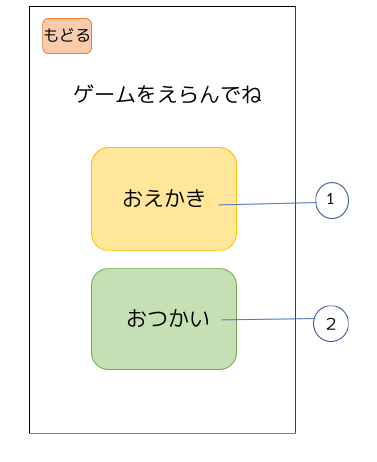
\includegraphics {game.png}}
    \caption {ゲーム画面}
    \label{game}
    \end{center}
\end{figure}

\begin{enumerate}
  \renewcommand{\labelenumi}{\textcircled{\scriptsize \theenumi}}
\item おえかき\\
  おえかきの矩形領域をタップするとお絵描きの詳細画面へ遷移します。
\item おつかい\\
  おつかいの矩形領域をタップするとおつかいのゲーム画面へ遷移します。
\end{enumerate}

\subsubsection{おえかき}
図\ref{oekaki}におえかきの詳細画面を示します。\\
画面上のボタンをタップすることでおえかきのモードを選択することができます。\\

\begin{figure}[H]
    \begin{center}
    \resizebox{8cm}{!}{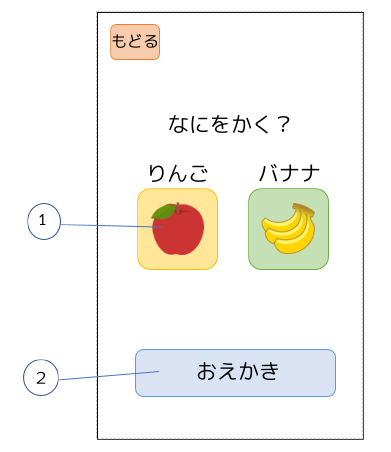
\includegraphics {oekaki.png}}
    \caption {おえかき画面}
    \label{oekaki}
    \end{center}
\end{figure}

\begin{enumerate}
  \renewcommand{\labelenumi}{\textcircled{\scriptsize \theenumi}}
\item イラストボタン\\
  イラストのボタンをタップすることで図\ref{illustration}のようにタップしたイラストを閲覧しながらのおえかきができます。
\item おえかきボタン\\
  おえかきのボタンをタップすることでおえかきの図\ref{oekaki2}のゲーム画面に遷移し、自由におえかきができます。
\end{enumerate}

\begin{figure}[H]
    \begin{center}
    \resizebox{8cm}{!}{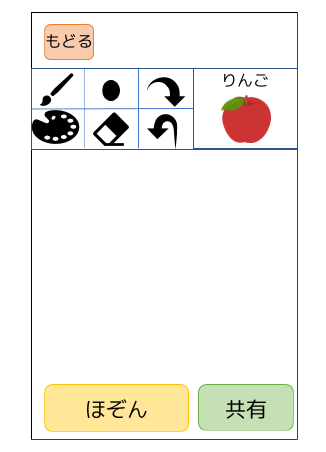
\includegraphics {illustration.png}}
    \caption {イラスト}
    \label{illustraion}
    \end{center}
\end{figure}

\begin{figure}[H]
    \begin{center}
    \resizebox{8cm}{!}{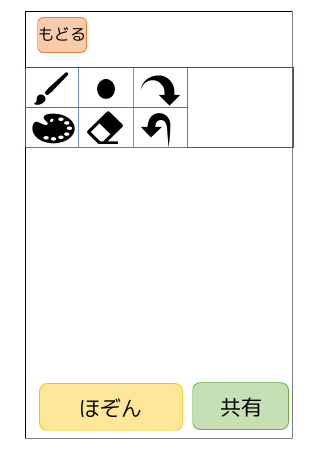
\includegraphics {oekaki2.png}}
    \caption {おえかき}
    \label{oekaki2}
    \end{center}
\end{figure}

\subsubsection{おつかい}
図\ref{otukai1}におつかいの詳細画面を示します。\\
おつかいは作りたい料理を選択し、その料理に必要な材料をお店から買ってくるゲームです。\\

\begin{figure}[H]
    \begin{center}
    \resizebox{8cm}{!}{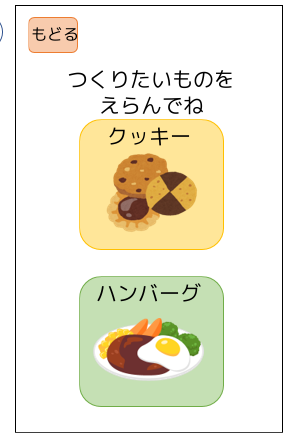
\includegraphics {otukai.png}}
    \caption {おつかい}
    \label{otukai1}
    \end{center}
\end{figure}

図\ref{otukai1}の料理のイラストボタンをタップするとその料理の材料画面(図\ref{material})に遷移します。材料画面(図\ref{material})のもどるボタンをタップすると図\ref{otukai1}にもどります。おつかいのボタンをタップするとお店の画面(図\ref{shop})へ遷移します。

\begin{figure}[H]
    \begin{center}
    \resizebox{8cm}{!}{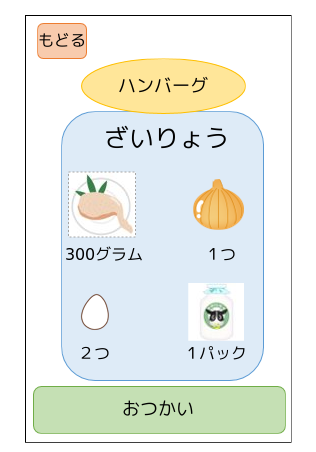
\includegraphics {material.png}}
    \caption {材料画面}
    \label{material}
    \end{center}
\end{figure}

お店のイラストボタンをタップすることでお店に置いている食材画面(図\ref{shop_material})へ遷移します。食材画面(図\ref{shop_material})のもどるボタンをタップすることでお店の画面(図\ref{shop})へ遷移します。

\begin{figure}[H]
    \begin{center}
    \resizebox{8cm}{!}{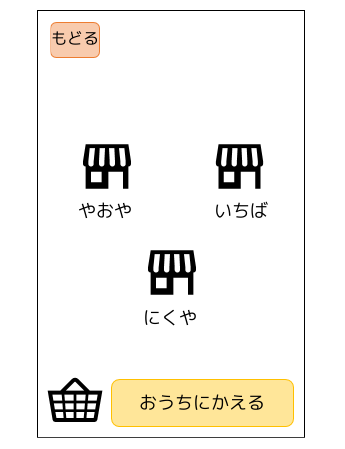
\includegraphics {shop.png}}
    \caption {お店}
    \label{shop}
    \end{center}
\end{figure}

食材画面(\ref{shop_material})の食材のイラストをタップすることで材料の中にタップした食材が1つずつ格納されます。かごのイラストボタンをタップすることで持っている材料を確認することができます。食材画面(\ref{shop_material})のもどるボタンをタップするとお店の画面(図\ref{shop})遷移します。
お店の画面(図\ref{shop})のおうちへと書かれたボタンをタップするとおうち画面(図\ref{myhome})へ遷移します。

\begin{figure}[H]
    \begin{center}
    \resizebox{8cm}{!}{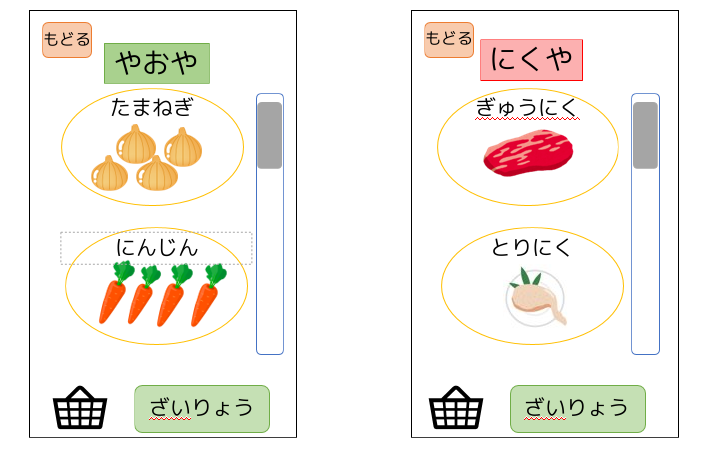
\includegraphics {shop2.png}}
    \caption {食材画面}
    \label{shop_material}
    \end{center}
\end{figure}
図\ref{myhome}はおうち画面を示します。\\

\begin{figure}[H]
    \begin{center}
    \resizebox{8cm}{!}{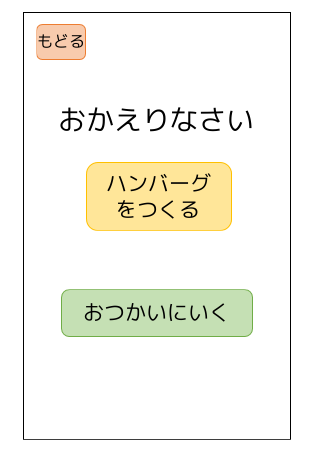
\includegraphics {go_home.png}}
    \caption {おうち画面}
    \label{myhome}
    \end{center}
\end{figure}

材料が揃っている場合、おうち画面(図\ref{myhome})のつくるボタンをタップするとできあがり画面(図\ref{completion})へ遷移します。

\begin{figure}[H]
    \begin{center}
    \resizebox{8cm}{!}{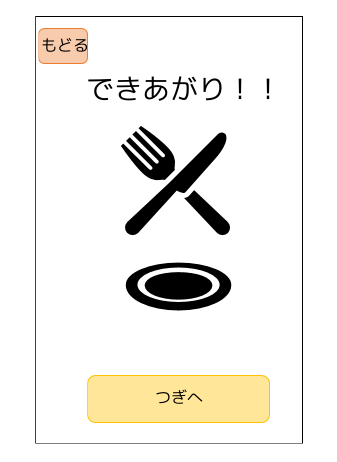
\includegraphics {completion.png}}
    \caption {できあがり画面}
    \label{completion}
    \end{center}
\end{figure}

材料が揃っていない場合、図\ref{otukai6}のように「材料が足りないよ」と表示され、閉じるボタンをタップするとおうち画面(図\ref{myhome})へ遷移します。おうち画面(図\ref{myhome})のおつかいボタンをタップするとお店の画面(図\ref{shop})遷移します。

\begin{figure}[H]
    \begin{center}
    \resizebox{8cm}{!}{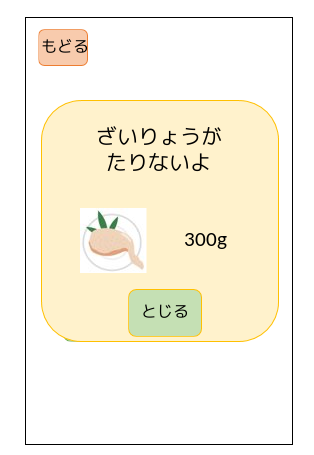
\includegraphics {lack.png}}
    \caption {材料が足りない場合}
    \label{otukai6}
    \end{center}
\end{figure}

\end{document}
